
% \section{Грамматический разбор}
% \label{pass:parsing}

% \section{Парсер Пратта}
% \label{pass:parsing:pratt}
% Парсер Пратта использует комбинацию циклов и рекурсивных вызовов функций.
% Есть хорошая статья, в которой приводится реализация данного парсера на языке Rust\cite{matklad_pratt_parsers}.

% Парсер Пратта для инфиксных операторов упрощенно работает по следующему принципу: 

% % \begin{lstlisting}[language=python, caption={Псевдокод алгоритма парсера Пратта}]
% % def parse_expr(state, max_precedence, flags) -> expr, err:
% %     left: Expr
    
% % \end{lstlisting}

% \begin{enumerate}
%     \item Начало определения рекурсивной функции \verb|parse_expr|, 
%     принимающей параметры состояния разбора \verb|state| и максимального значения порядка следования \verb|max_precedence|

%     \begin{itemize}
%         \item Пусть \verb|left: Expr| - переменная типа \verb|Expr|

%         \item В \verb|left| записывается первый аргумент или выходим с ошибкой, если его нет или он является именем типа

%         \item\label{pratt:alg:loop} Пока есть следующий за аргументом бинарный оператор, удовлетворяющий ограничениям порядка следования и ассоциативности:

%         \begin{itemize}
%             \item Разбираем оператор записываем в переменную \verb|op: Expr|

%             \item\label{pratt:alg:rec-call} Разбираем правый операнд выражения рекурсивным вызовом функции \verb|parse_expr|, 
%             со значением \verb|max_precedence| равным порядку следования оператора в переменной \verb|op|

%             \item Записываем в \verb|left| значение переменной \verb|op|
%         \end{itemize}
%     \end{itemize}

%     \item Конец определения функции \verb|parse_expr|
% \end{enumerate}


% Рекурсивные вызовы[\ref{pratt:alg:rec-call}] в алгоритме сами по себе разбирают цепочки операторов с убывающем номером порядка следования
% (или одинаковым при условии ассоциативности справа на лево). 
% Синтаксические деревья полученные после разбора таких операторов, являются наклоненными направо, как показано на диаграмме[\ref{pratt:right-lean-diag}].

% Тогда как цикл[\ref{pratt:alg:loop}] в алгоритме сам по себе разбирает цепочки операторов с оставшимися после рекурсивного вызова номерами порядка следования, 
% т.е. возрастающими или одинаковыми при условии ассоциативности слева на право. 
% Синтаксические деревья полученные после разбора таких операторов, являются наклоненными налево, как показано на диаграмме[\ref{pratt:left-lean-diag}].


% \begin{figure}[h!]
%     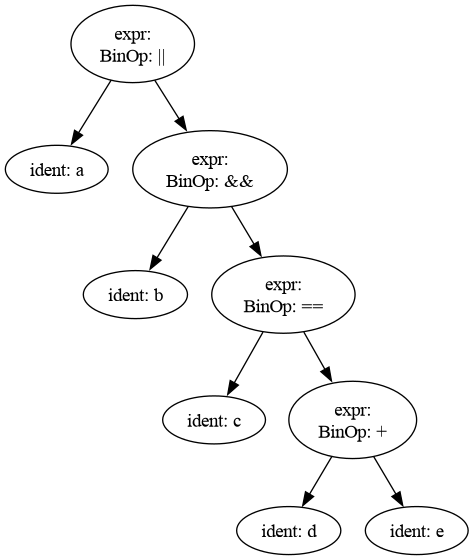
\includegraphics[width=\textwidth,height=\textheight,keepaspectratio]{right-lean-diag.png}
%     \centering
%     \caption{AST цепочки операторов с убывающим номером порядка следования}
%     \label{pratt:right-lean-diag}
% \end{figure}

% \begin{figure}[h!]
%     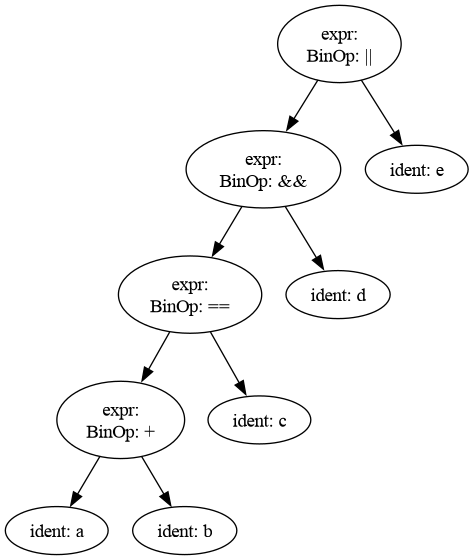
\includegraphics[width=\textwidth,height=\textheight,keepaspectratio]{left-lean-diag.png}
%     \centering
%     \caption{AST цепочки операторов с возрастающим номером порядка следования}
%     \label{pratt:left-lean-diag}
% \end{figure}


% \FloatBarrier




\clearpage
\section{Грамматический разбор}
\label{pass:parsing}

Далее будет рассмотрен грамматический разбор или парсинг потока токенов, получаемого после прохода лексера.
Грамматический разбор - процесс превращения потока(последовательности) лексических единиц в синтаксическое дерево, рассматриваемое далее[\ref{parsing:ast}].
Разбор производится методом рекурсивного спуска, который рассматривается далее[\ref{parsing:rec-desc}]. Для разбора выражений используется парсер Пратта, рассмотренные далее в параграфе[\ref{pass:parsing:pratt}].

\section{Метод рекурсивного спуска}
\label{parsing:rec-desc}

Метод рекурсивного спуска заключается в применении взаимно рекурсивных функций для разбора последовательно лексем.
Каждая рекурсивная функция соответствует какому-то нетерминалу грамматики языка.
Среди функций разбора, есть нерекурсивные, соответствующие некоторым терминалам языка.

Различают предсказывающие и спекулятивные(парсеры с возвратом) парсеры рекурсивного спуска:
\begin{itemize}
\item предсказывающие по конкретному токену(токенам) могут определить, какое правило разбора применить дальше. Работают за линейное время.
\item спекулятивные последовательно пробуют несколько правил разбора, пока одно не сработает. Такие парсера потенциально(в худшем случае) работают за экспоненциальное время.
\end{itemize}

В данной работе реализован предсказывающий парсер, однако можно заметить, 
что в коде(например функции разбора определений[\ref{extras:parse_decl}]) используются спекулятивные вызовы(оборачиваемые в макрос \verb|PARSER_OPTIONAL|[\ref{parsing:parser-optional-expl}]).
Подобные вызовы используют только терминальные функции, вследствие чего подобный вызов аналогичен обычной проверки условия, например на то, что текущий токен является пунктуатором.

Например, следующее условие с вызовом:

\begin{lstlisting}[language=c]
if (IS_OK(PARSER_OPTIONAL(c_parse_t_punct_kind(state, C_PUNCT_EQUAL, &tok)))) {
    ...
}
\end{lstlisting}

эквивалентно условию:

\begin{lstlisting}[language=c]
if (tok->kind == C_TOKEN_KIND_PUNCT && tok->t_punct.punct_kind == C_PUNCT_EQUAL) {
    *tok = parser_advance(state);
    ...
}
\end{lstlisting}


\section{Структура парсера и его методы}

Также как на этапе лексического разбора[\ref{pass:lexing}] на данном этапе имеется структура, содержащая состояние разбора.

\begin{lstlisting}[language=c]
struct_def(ParserState, { ... })
\end{lstlisting}

Данная структура содержит информацию о:
\begin{itemize}
    \item последовательности разбираемых токенов
    \item номер текущего разбираемого токена
    \item текущее окружение, для разрешения имен
    \item флаг, указывающий, откладывает ли парсер разбор контекстно зависимых частей языка
    \item флаг, указывающий, находится ли парсер в режиме ошибки
    \item аллокаторы для строк и элементов AST
    \item функции обработки ошибок аллокации и возникающих при разборе
\end{itemize}



У парсера имеются методы для сигнализации и обработки ошибок.

Когда какая-нибудь функция разбора возвращается ошибку, она дополнительно может привести сообщение об ошибке с помощью макросов:

\begin{lstlisting}[language=c, caption={Макросы сообщения об ошибке}]
#define parser_error(state, _msg, args...) ...
#define parser_error_pos(state, _pos, _msg, args...) ...
#define parser_error_expected(state, expected, args...) ... 
\end{lstlisting}

При выполнении эти макросы ставят флаг \verb|ParserState::was_error|, сообщая дальнейшим процессам о наличии ошибки.
При этом ошибка устанавливается, только если нет активной ошибки (флаг \verb|ParserState::was_error| равен \verb|false|), так в цепочке ошибок до конца дойдет только первая встретившаяся, 
находящаяся на глубине стека вызовов и соответственно самая частная, зачастую несущая информацию о том, что пользователю надо изменить в программе, чтобы та была корректной.

В добавок к этому функции разбора возвращают статут разбора при завершении:
\begin{lstlisting}[language=c, caption={Виды статуса возвращаемого значения парсера}]
enum_def(ParsingError, 
    PARSING_ERROR_OK,
    PARSING_ERROR_NONE,
    PARSING_ERROR_EOF,
)
#define PARSING_ERROR(ERR) ((ParsingError)PARSING_ERROR_##ERR)
\end{lstlisting}

Для обработки вышеперечисленного вызывающими функциями(callers) используются следующие макросы: 
\begin{lstlisting}[language=c, caption={Вспомогательные макросы обработки состояния разбора}]
#define PARSER_ALLOC_HANDLE(f) ...
#define PARSER_TRY(p) ... 
#define PARSER_OPTIONAL(p) ...
#define PARSING_OK(state) ...
#define PARSING_NONE(state, prev) ...
\end{lstlisting}

Где
\begin{itemize}
    \item \verb|PARSER_ALLOC_HANDLE| - при неудачном завершении вызываемого, вызывает обработчик ошибок аллокации, строенный в парсер
    \item \verb|PARSER_TRY| - при неудачном завершении вызываемого, отдаст ошибку далее по стеку
    \item\label{parsing:parser-optional-expl} \verb|PARSER_OPTIONAL| - при неудачном завершение вызываемого, "заглушит" ошибку
    \item \verb|PARSER_OK| - выйдет из функции с "успехом" 
    \item \verb|PARSER_NONE| - выйдет из функции с "неудачей", восстановив состояние парсера до начала разбора текущей функцией
\end{itemize}

% \beginminteddef{c}
% \end{minted}




\section{Абстрактное синтаксическое дерево}
\label{parsing:ast}

Грамматика языка Си приведена в CFG форме, каждый нетерминал грамматики по сути является элементом синтаксического дерева, 
однако после разбора такое дерево сдержит множество излишних деталей, подробностей разбора.
Разработанное абстрактное синтаксическое дерево(AST) является "выжимкой" из синтаксического дерева и будет рассмотрено далее.

Абстрактное синтаксическое дерево, получаемое в ходе грамматического разбора, состоит из элементов(nodes).
Как и в случае с лексером тип \verb|C_Ast_Node| тоже является типом объединения частных типов, которые зачастую в свою очередь тоже являются объединениями дочерних типов.
Данная иерархия будет рассмотрена далее, полный код синтаксического дерева можно посмотреть в приложении[\ref{extras:c_ast}].

Самый общий тип иерархии тип \verb|C_Ast_Node|, далее приведено определение его структуры:


\begin{lstlisting}[language=c, caption={Структура элемента AST}, label={parsing:ast:node-struct}]
#define C_AST_NODE_BASE \
    C_Ast_NodeKind kind;\
    C_ParserSpan span;\

struct_def(C_Ast_Node, {
    union {
    struct {
        C_AST_NODE_BASE
    };
        C_Ast_Ident ident;
        C_Ast_Literal lit;
        C_Ast_Expr expr;
        C_Ast_Stmt stmt;
        C_Ast_Type ty;
        C_Ast_Decl decl;
        C_Ast_TranslationUnit tr_unit;
    #ifdef EXTENDED_C
        C_Ast_AtDirective at_directive;
    #endif // EXTENDED_C
    };
})
\end{lstlisting}

Элементами его являются:
\begin{itemize}
    \item идентификатор
    \item литерал
    \item выражение
    \item утверждения
    \item имя-типа
    \item определение
    \item единица-трансляции
    \item @ директива
\end{itemize}

При разборе ноды дерева сохраняются в отдельную арену памяти(далее \verb|ParserState::ast_arena|).

Замечание: \verb|C_AST_Node| - тип переменной длины, для конкретной ноды ее размер равен размеру частной ноды,
т.е. чтобы скопировать или записать существующую ноду надо сначала понять, какого она типа.

Для построения нод используются вспомогательные макросы:
\begin{lstlisting}[language=c]
#define make_node(state, out_node, KIND_SUFF, args...) {\
    PARSER_ALLOC_HANDLE(allocator_alloc_T(&state->ast_alloc, typeof(**out_node), out_node));\
    **out_node = ((typeof(**out_node)) {.kind = C_AST_NODE_KIND_##KIND_SUFF, ##args });\
}
#define make_node_type(state, out_node, TYPE_KIND_SUFF, args...) ...
#define make_node_decl(state, out_node, DECL_KIND_SUFF, args...) ...
#define make_node_stmt(state, out_node, STMT_KIND_SUFF, args...) ...
#define make_node_expr(state, out_node, EXPR_KIND_SUFF, args...) ...
#define make_node_lit(state, out_node, LIT_KIND_SUFF, args...) ...
\end{lstlisting}

Данные макросы выделяют достаточное кол-во памяти под данный тип элемента AST, и заполняют его приведенными полями.

% \section{@ директивы}
Отдельным элементом AST стоят @ директивы, добавленные в расширении.
Далее привожу их грамматику:

% \clearpage
% \label{pass:parsing:at-directive}

Привожу грамматику директив, встраиваемою в грамматику Си, приведенную в стандартах\cite{c99_std}:
\begin{lstlisting}[language=bash, caption={Грамматика @ директив}, label={parsing:at-directive:grammar}]
at-directive:
    @ directive-name
    @ directive-name (at-directive-args)

at-directive-args:
    at-directive-args at-directive-arg     

at-directive-arg:
    identifier-or-literal

identifier-or-literal:
    identifier
    literal

literal:
    constant
\end{lstlisting}

\section{Контекстная зависимость грамматики Си}
\label{parsing:context-dep}

Грамматика фразовых структур языка Си, приведенная в стандарте\cite{c99_std} (Annex A, 2. Phrase structure grammar),
по большей части является контекстно свободной, однако зависимость от контекста, можно показать на следующем примере(пример взять из статьи\cite{eli_c_cs}):

\begin{lstlisting}[language=c]
(T) * x;
\end{lstlisting}

В зависимости от того, что такое \verb|T| (идентификатор или имя типа) данное выражение может быть разобрано по разному:
как умножение двух переменных
\begin{lstlisting}[language=c]
T * x;
\end{lstlisting}
или как оператор приведения к типу (T), примененному к разыменовыванию указателя \verb|x|
\begin{lstlisting}[language=c]
(T) (*x);
\end{lstlisting}

Это проиллюстрировано в следующем изображение[\ref{parsing:gram-dep-diag}]:
\begin{figure}[h!]
    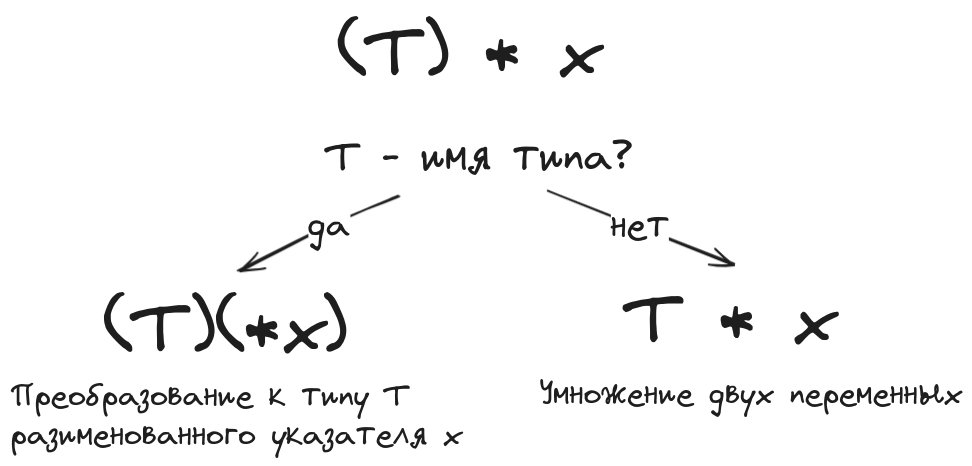
\includegraphics[width=\textwidth,height=\textheight,keepaspectratio]{gram-dep-diag.png}
    \centering
    \caption{Зависимость грамматики выражений Си от контекста}
    \label{parsing:gram-dep-diag}
\end{figure}
\FloatBarrier


Далее в Си есть понятие затенения(shadowing) имен. 
Следующий пример демонстрирует, что имя типа может быть затенено (использовался компилятор gcc):

\begin{lstlisting}[language=c, caption={Пример затенения имен}, label={parsing:name-shadowing-ex}]
typedef int Foo2;

void test_type_name() {
    int Foo2 = 3;
    int x;
    x = (Foo2) + x;
}
\end{lstlisting}

\verb|Foo2| внутри функции \verb|test_type_name| затеняет \verb|typedef| определение, и выражение \verb|(Foo2) + x| разбирается как сумма, 
а не приведение к типу \verb|Foo| и унарный плюс.

Так что для корректного разбора выражений языка Си, нужна система разрешения имен.

Данная система выполнена в виде стека таблиц символов(далее тип \verb|C_Environment|).
Внизу стека лежит глобальная таблица символов, где хранятся определения типов и функций. Далее по стеку идут локальные таблицы символов, соответствующие вложенным блокам кода(scopes).

\begin{lstlisting}[language=c, caption={Определения структур сивола и окружения}, label={parsing:env-struct}]
typedef str_t C_Symbol;
typedef hashmap_T(C_Symbol, C_SymbolData) C_SymbolTable;

struct_def(C_SymbolData, {
    C_Ast_Node *node;
    ...
})

typedef darr_T(C_SymbolTable *) C_Environment;
\end{lstlisting}

Для разрешения имени функция \verb|c_environment_get_sym_data| идет по стеку сверху вниз, проверяя принадлежит ли имя текущему блоку.
Так при определении нового имени в текущем блоке, оно перекроет имена находящиеся в нижележащих блоках. 

\begin{lstlisting}[language=c, caption={Определение функции разрешения имени символа}, label={parsing:get-sym-data-def}]
C_SymbolData NLB(*)
c_environment_get_sym_data(C_Environment env, C_Symbol sym) {
    C_SymbolData *data = nullptr;
    for (isize_t i = (isize_t)darr_len(env) - 1; i >= 0; i -= 1) {
        data = hashmap_get(**darr_get_T(C_SymbolTable *, env, i), &sym);
        if (data != nullptr) {
            break;
        }
    }
    return data;
}
\end{lstlisting}








\section{Функции грамматического разбора}

Рассмотрим самую внешнюю функцию грамматического разбора - функцию разбора единицы трансляции языка EC.
\begin{lstlisting}[language=c, caption={Функция разбора единицы трансляции}, label={parsing:ec-parse-tr-unit}]
ParsingError
ec_parse_translation_unit(ParserState *state, EC_Ast_TranslationUnit **out_tr_unit) {
    auto prev = parser_save(state);

    darr_t tr_unit_items;
    PARSER_ALLOC_HANDLE(darr_new_cap_in_T(EC_Ast_TrUnitItem *, 16, &state->ast_alloc, &tr_unit_items));

    EC_Ast_TrUnitItem *item = nullptr;
    while (parser_peek(state)->kind != C_TOKEN_KIND_EOF) {
        PARSER_ALLOC_HANDLE(darr_reserve_cap(&tr_unit_items, 1));
        if (parser_peek_punct_kind(state, C_PUNCT_AT)) {
            if (IS_ERR(ec_parse_at_directive(state, (EC_Ast_AtDirective **)&item))) {
                PARSING_NONE(state, &prev);
            }
        } else if (IS_ERR(c_parse_declaration(state, (C_Ast_Decl **)&item))) {
            PARSING_NONE(state, &prev);
        }

        *darr_get_unchecked_T(EC_Ast_TrUnitItem *, tr_unit_items, darr_len(tr_unit_items)) = item;
        tr_unit_items->len += 1;
    }

    make_node(state, out_tr_unit, EC_TR_UNIT, 
            .items = tr_unit_items,
            .span = parser_span_from_save(state, &prev),
        );

    return PARSING_ERROR(OK);
}
\end{lstlisting}

Данная функция в цикле, пока есть неразобранные токены, по первому токену в зависимости о того, 
является ли он символом @ или нет, разбирает директиву или определение языка Си. 
Разобранные элементы добавляются в список элементов единицы трансляции.
В конце конструируется элемент AST с помощью макроса \verb|make_node| с использованием данного списка элементов.

Так как EC откладывает разбор выражений, на данном этапе глобальная таблица символов не конструируется.

Директивы разбираются согласно приведенной выше грамматики[\ref{parsing:at-directive:grammar}].
Функции разбора определений можно посмотреть в приложении[\ref{extras:parse_decl}].

Для полноты рассмотрим также функцию разбора элементов составного утверждения вида

\begin{lstlisting}[language=c]
{
    ...
}
\end{lstlisting}

\begin{lstlisting}[language=c, caption={Функция разбора элеметов составного утверждения}, label={parsing:c-parse-block}]
ParsingError
c_parse_block(ParserState *state, C_SymbolTable *scope, darr_T(C_Ast_BlockItem *) *out_items) {
    auto prev = parser_save(state);
    if (*scope == nullptr) {
        PARSER_ALLOC_HANDLE(hashmap_new_cap_in_T(C_Symbol, C_SymbolData, 8, &state->ast_alloc, scope));
    }
    darr_t items = nullptr;
    PARSER_ALLOC_HANDLE(darr_new_cap_in_T(C_Ast_BlockItem *, 8, &state->ast_alloc, &items));
    
    c_environment_push_scope(&state->env, scope);

    while (true) {
        if (parser_peek_punct_kind(state, C_PUNCT_RIGHT_BRACE)) {
            break;
        }
        if (parser_peek_punct_kind(state, C_PUNCT_SEMI_COLON) || 
            c_token_is_type_name_beginning(state->env, parser_peek(state))) 
        {
            C_Ast_Decl *block_item = nullptr;
            PARSER_TRY(c_parse_decl(state, &block_item))
            PARSER_ALLOC_HANDLE(darr_push(&items, &block_item));
            if (state->collect_symbols) {
                if (!c_parser_scope_collect_symbols_decl(state, scope, block_item)) {
                    PARSING_NONE(state, &prev);
                }
            }
        } else {
            C_Ast_Stmt *block_item = nullptr;
            PARSER_TRY(c_parse_stmt(state, &block_item))
            PARSER_ALLOC_HANDLE(darr_push(&items, &block_item));
        }
    }

    c_environment_pop_scope(&state->env);
    *out_items = items;

    PARSING_OK(state);
}
\end{lstlisting}
 

В данном случае разбор не откладывается и выполняется линейно с использованием окружения \verb|state->env|, рассмотренного ранее[\ref{parsing:context-dep}]. 
Т.к. составные утверждения вводят новую область видимости, данная функция создаёт новую таблицу символов, 
реализующую локальную область видимости (local scope), и добавляет ее в стек окружения \verb|state->env|. 

При разборе эта функция последовательно заполняет таблицу символов с помощью вызовов функций \verb|c_parser_scope_collect_symbols_decl| и тут же использует ее для последующего разбора.

Используемая в цикле функция \verb|c_token_is_type_name_beginning| проверяет, является ли токен началом имени типа, используя окружение \verb|state->env|.
В зависимости от этого выбирается, что разбирать дальше определение или утверждение.

Подробно в данной главе я рассмотрю только разбор выражений, некоторые функции разбора определений и утверждений можно посмотреть в соответствующих приложениях \ref{extras:parse_decl} и \ref{extras:parse_stmt}.

% \section{Идентификаторы и литералы}

% \beginminteddef{c}
% struct_def(C_Ast_Ident, {
%     C_AST_NODE_BASE

%     str_t name;
% })

% enum_def(C_Ast_LiteralKind, 
%     C_AST_LITERAL_KIND_INVALID,
%     C_AST_LITERAL_KIND_STRING,
%     C_AST_LITERAL_KIND_CHAR,
%     C_AST_LITERAL_KIND_NUMBER,
%     C_AST_LITERAL_KIND_COMPOUND,
% ) 
% \end{minted}

% \begin{itemize}
%     \item STRING, NUMBER, CHAR совпадают с соответствующими токенами
%     \item COMPOUND - составной литерал, например \verb|(str_t) {.ptr = nullptr, .byte_len = 0}|
% \end{itemize}

\clearpage
\section{Выражения}

Следующая диаграмма[\ref{parsing:expr-ast-diag}] иллюстрирует структуру AST для выражений языка Си: 

% \begin{tikzpicture}[
% roundnode/.style={ellipse, draw=black!60, fill=green!0, very thick, minimum size=7mm},
% squarednode/.style={rectangle, draw=red!60, fill=red!5, very thick, minimum size=5mm},
% ]
% %Nodes
% \node[roundnode]      (maintopic)                              {Expr};
% \node[roundnode]        (unop)       [below=of maintopic] {UnOp};
% \node[roundnode]      (binop)       [below=of maintopic] {BinOP};
% \node[roundnode]        (lowercircle)       [below=of maintopic] {4};

% %Lines
% \draw[->] (maintopic.north) -- (binop.south);
% \draw[->] (maintopic.north) -- (unop.south);
% % \draw[->] (uppercircle.south) -- (maintopic.north);
% % \draw[->] (rightsquare.south) .. controls +(down:7mm) and +(right:7mm) .. (lowercircle.east);
% \end{tikzpicture}


\begin{figure}[h!]
    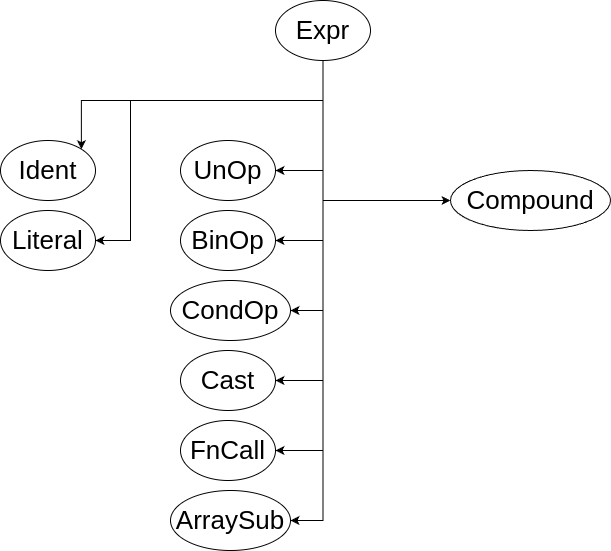
\includegraphics[width=\textwidth]{expr-ast.png}
    \centering
    \caption{AST выражения Си}
    \label{parsing:expr-ast-diag}
\end{figure}

% \begin{lstlisting}[language=c]
% enum_def(C_Ast_ExprKind, 
%     C_AST_EXPR_KIND_INVALID,
%     C_AST_EXPR_KIND_IDENT,
%     C_AST_EXPR_KIND_LITERAL,
%     C_AST_EXPR_KIND_UNOP,
%     C_AST_EXPR_KIND_BINOP,
%     C_AST_EXPR_KIND_CONDOP, // ?:
%     C_AST_EXPR_KIND_CAST,
%     C_AST_EXPR_KIND_FN_CALL,
%     C_AST_EXPR_KIND_ARRAY_,
%     C_AST_EXPR_KIND_COMPOUND, // expr, expr, ... expr
% )
% \end{lstlisting}

% \begin{itemize}
%   \item \verb|IDENT| - \verb|x|
%   \item \verb|LITERAL| - \verb|3|
%   \item \verb|UNOP| - \verb|-x|
%   \item \verb|BINOP| - \verb|x + y|
%   \item \verb|CONDOP| - \verb|x > y ? a : b|
%   \item \verb|CAST| - \verb|(T) expr|
%   \item \verb|FN_CALL| - \verb|f(e1, e2, e3)|
%   \item \verb|ARRAY_| - \verb|arr[x]|
%   \item \verb|COMPOUND| - \verb|e1, e2, e3|
% \end{itemize}

% % \beginminteddef{c}
% % \end{minted}

% \subsection{Разбор выражений}

Для разбора выражений используется парсер Пратта, который хорошо сочетается с разбором методом рекурсивного спуска.
Данный парсер использует таблицу приоритета и ассоциативности операторов. Данная таблица приведена в определениях[\ref{extras:c_defs}].

Операторы разделены на три группы: префиксные, инфиксные, постфиксные.
Отдельно обрабатывается тернарный условный оператор \verb|?:|.

Для каждого из этих групп есть функция, распознающая оператор по типу с ограничением по приоритету.

\begin{lstlisting}[language=c, caption={Функции разбора операторов}, label={parsing:expr:parse-op-headers}]
ParsingError
c_parse_expr_op_infix_prec_rb(ParserState *state, C_Ast_ExprBinOp **out_binop, u8_t max_precedence, bool is_strict_precedence);
ParsingError
c_parse_expr_op_prefix_prec_rb(ParserState *state, C_Ast_ExprUnOp **out_unop, u8_t max_precedence, bool is_strict_precedence);
ParsingError
c_parse_expr_op_postfix_prec_rb(ParserState *state, C_Ast_ExprUnOp **out_unop, u8_t max_precedence);
ParsingError
c_parse_expr_op_tern_cond_prec_rb(ParserState *state, C_Ast_ExprCondOp **out_tern, u8_t max_precedence, bool is_strict_precedence);
\end{lstlisting}

Замечание: числовое значение приоритета идет(возрастает) в порядке убывания приоритета[\cite{cppref_op_prec}].

Так например \verb|c_parse_expr_op_infix_prec_rb| проверяет принадлежит ли пунктуатор множеству инфиксных операторов,
затем если приоритет оператора ниже минимального приоритета, то функция выходит с ошибкой, 
если приоритет совпадает с минимальным, то проверяется ассоциативность, если оператор группируется слева на право, то функция выходит с ошибкой.
Также существует флаг \verb|STRICT_PRECEDENCE|, отсекающий случай равных приоритетов.

Следующие функции разбирают выражения, имплементацию их можно посмотреть в приложении[\ref{extras:parse_expr}].

\begin{lstlisting}[language=c, caption={Заголовки функции разбора выражений}, label={parsing:expr:parse-expr-headers}]
ParsingError
_c_parse_expr(ParserState *state, C_Ast_Expr **out_expr, u8_t max_precedence, C_ExprFlags flags);
ParsingError
c_parse_expr_assign(ParserState *state, C_Ast_Expr **out_expr);
ParsingError
c_parse_expr_cond(ParserState *state, C_Ast_Expr **out_expr);
ParsingError
c_parse_expr(ParserState *state, C_Ast_Expr **out_expr);
\end{lstlisting}

Также, поскольку грамматика выражений Си является контекстно зависимой, то используется окружение(рассмотренное выше[\ref{parsing:context-dep}]), для разрешения имен,
в частности для проверки является ли имя идентификатора именем типа или нет.

Графическое изображение AST выражения см. далее[\ref{pratt:right-lean-diag}] и [\ref{graphviz:expr}]

\section{Алгоритм парсера Пратта}
\label{pass:parsing:pratt}

Парсер Пратта использует комбинацию циклов и рекурсивных вызовов функций.
Есть хорошая статья, в которой приводится реализация данного парсера на языке Rust\cite{matklad_pratt_parsers}.

Парсер Пратта для инфиксных операторов упрощенно работает по следующему принципу: 

% \begin{lstlisting}[language=python, caption={Псевдокод алгоритма парсера Пратта}]
% def parse_expr(state, max_precedence, flags) -> expr, err:
%     left: Expr
    
% \end{lstlisting}

\begin{enumerate}
    \item Начало определения рекурсивной функции \verb|parse_expr|, 
    принимающей параметры состояния разбора \verb|state| и максимального значения порядка следования \verb|max_precedence|

    \begin{itemize}
        \item Пусть \verb|left: Expr| - переменная типа \verb|Expr|

        \item В \verb|left| записывается первый аргумент или выходим с ошибкой, если его нет или он является именем типа

        \item\label{pratt:alg:loop} Пока есть следующий за аргументом бинарный оператор, удовлетворяющий ограничениям порядка следования и ассоциативности:

        \begin{itemize}
            \item Разбираем оператор записываем в переменную \verb|op: Expr|

            \item\label{pratt:alg:rec-call} Разбираем правый операнд выражения рекурсивным вызовом функции \verb|parse_expr|, 
            со значением \verb|max_precedence| равным порядку следования оператора в переменной \verb|op|

            \item Записываем в \verb|left| значение переменной \verb|op|
        \end{itemize}
    \end{itemize}

    \item Конец определения функции \verb|parse_expr|
\end{enumerate}


Рекурсивные вызовы[\ref{pratt:alg:rec-call}] в алгоритме сами по себе разбирают цепочки операторов с убывающем номером порядка следования
(или одинаковым при условии ассоциативности справа на лево). 
Синтаксические деревья полученные после разбора таких операторов, являются наклоненными направо, как показано на диаграмме[\ref{pratt:right-lean-diag}].

Тогда как цикл[\ref{pratt:alg:loop}] в алгоритме сам по себе разбирает цепочки операторов с оставшимися после рекурсивного вызова номерами порядка следования, 
т.е. возрастающими или одинаковыми при условии ассоциативности слева на право. 
Синтаксические деревья полученные после разбора таких операторов, являются наклоненными налево, как показано на диаграмме[\ref{pratt:left-lean-diag}].


% \begin{figure}[h!]
%     \begin{figure}{.5\textwidth}
%         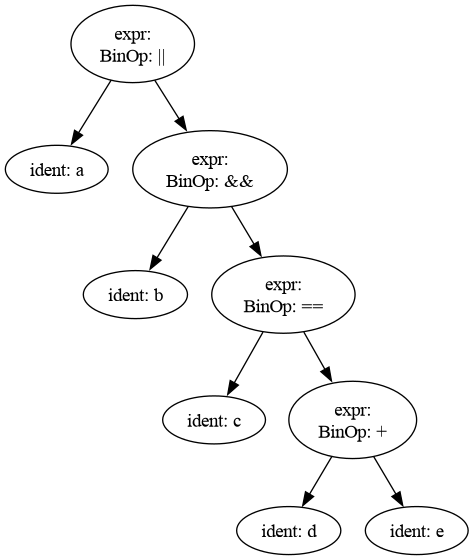
\includegraphics[width=.4\linewidth]{right-lean-diag.png}
%         \centering
%         \caption{AST цепочки операторов с убывающим номером порядка следования}
%         \label{pratt:right-lean-diag}
%     \end{figure}

%     \begin{figure}{.5\textwidth}
%         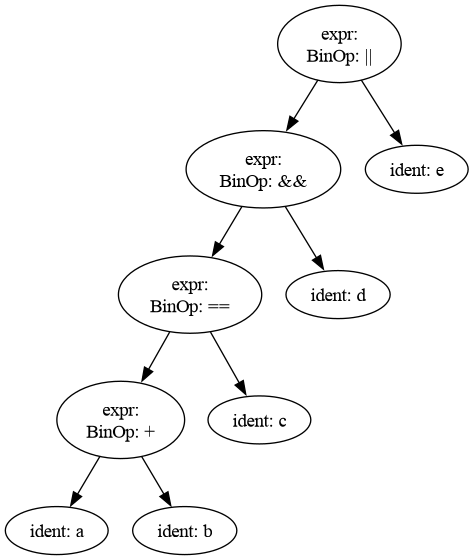
\includegraphics[width=.4\linewidth]{left-lean-diag.png}
%         \centering
%         \caption{AST цепочки операторов с возрастающим номером порядка следования}
%         \label{pratt:left-lean-diag}
%     \end{figure}
% \end{figure}

% \begin{figure}[h!]
%     \centering
%     \begin{minipage}{.5\textwidth}
%         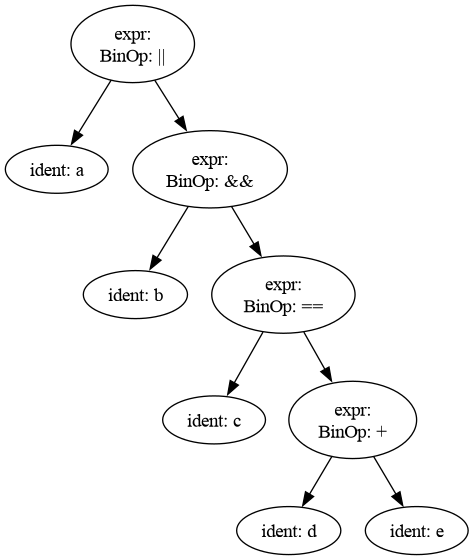
\includegraphics[width=.4\linewidth]{right-lean-diag.png}
%         \centering
%         \caption{AST цепочки операторов с убывающим номером порядка следования}
%         \label{pratt:right-lean-diag}
%     \end{minipage}
%     \begin{minipage}{.5\textwidth}
%         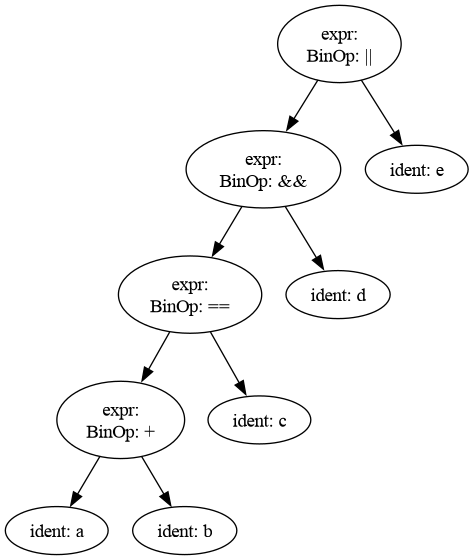
\includegraphics[width=.4\linewidth]{left-lean-diag.png}
%         \centering
%         \caption{AST цепочки операторов с возрастающим номером порядка следования}
%         \label{pratt:left-lean-diag}
%     \end{minipage}
% \end{figure}

\begin{figure}[h!]
    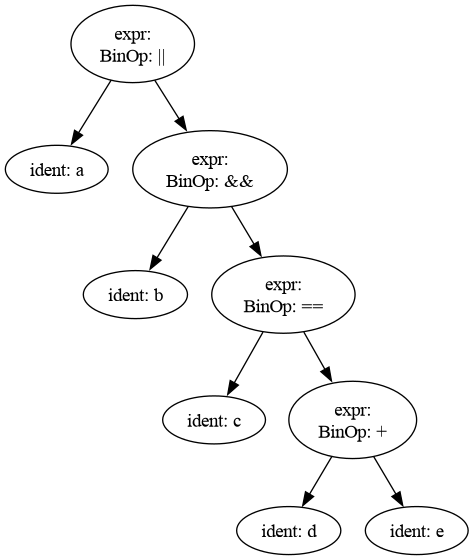
\includegraphics[width=.4\linewidth]{right-lean-diag.png}
    \centering
    \caption{AST цепочки операторов с убывающим номером порядка следования}
    \label{pratt:right-lean-diag}
\end{figure}
\begin{figure}[h!]
    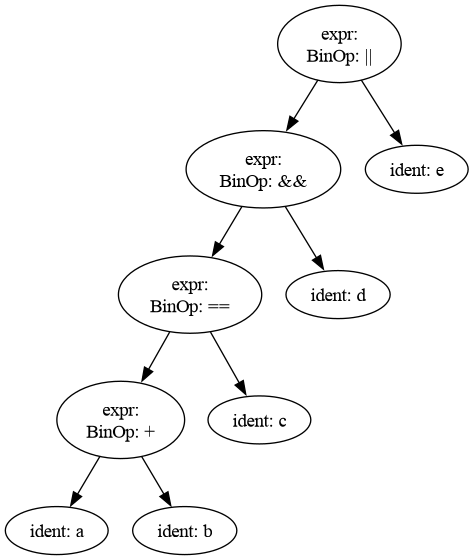
\includegraphics[width=.4\linewidth]{left-lean-diag.png}
    \centering
    \caption{AST цепочки операторов с возрастающим номером порядка следования}
    \label{pratt:left-lean-diag}
\end{figure}

\FloatBarrier


Комбинируя два этих подхода получаем всевозможные синтаксические деревья для выражений.

Подробнее данный алгоритм можно посмотреть в реализации функции \verb|_c_parse_expr| в приложении[\ref{extras:parse_expr}].



% \section{Определения}

% Виды нод типов:
% \beginminteddef{c}
% enum_def(C_Ast_TypeKind, 
%     C_AST_TYPE_KIND_INVALID,
%     C_AST_TYPE_KIND_IDENT,
%     C_AST_TYPE_KIND_POINTER,
%     C_AST_TYPE_KIND_ARRAY,
%     C_AST_TYPE_KIND_FUNCTION,
%     C_AST_TYPE_KIND_STRUCT,
%     C_AST_TYPE_KIND_UNION,
%     C_AST_TYPE_KIND_ENUM
% )
% \end{minted}

% Виды нод определений:
% \beginminteddef{c}
%     C_AST_DECL_KIND_INVALID,
%     C_AST_DECL_KIND_EMPTY, // ;;
%     C_AST_DECL_KIND_TYPE_DECL, // `struct(enum, union) A {};`
%     C_AST_DECL_KIND_VARIABLE, //  `struct A {} a;`, `int (*foo_p)(void), foo(void);`
%     C_AST_DECL_KIND_FN_DEF, // `int foo(void) {}`
%     C_AST_DECL_KIND_TYPEDEF, // typedef int Foo(void), Arr[3];
% \end{minted}


% Следующие функции разбирают определения, имплементацию их можно посмотреть в приложении[\ref{extras:parse_decl}]
% \beginminteddef{c}
% ParsingError
% c_parse_declarator(ParserState *state, C_Ast_Type **decl_ty_head, C_Ast_Type **decl_ty_leaf, C_Ast_Ident **decl_name);
% ParsingError
% c_parse_direct_declarator(ParserState *state, C_Ast_Type **decl_ty_head, C_Ast_Type **decl_ty_leaf, C_Ast_Ident **decl_name);
% ParsingError
% c_parse_record(ParserState *state, C_Ast_TypeKind struct_or_union_kind, C_Ast_TypeRecord **out_rec);
% ParsingError
% c_parse_type_specifier(ParserState *state, C_Ast_Type **out_ty);
% ParsingError
% c_parse_declaration(ParserState *state, C_Ast_Decl **out_decl);
% \end{minted}

% Функции \verb|c_parse_declarator|, \verb|c_parse_direct_declarator| взаимно рекурсивны, часть их задачи является разбор типов указателей массивов и функций, т.е. выражений вида:
% \mint{c}|int (*(*x)[3])(int a)| 

% Пример визуализации AST для такого определения см. далее[\ref{graphviz:decl}]


% \section{Утверждения}

% Виды утверждений:
% \beginminteddef{c}
% enum_def(C_Ast_StmtKind, 
%     C_AST_STMT_KIND_INVALID,
%     C_AST_STMT_KIND_EXPR,

%     C_AST_STMT_KIND_IF,
%     C_AST_STMT_KIND_SWITCH,

%     C_AST_STMT_KIND_LABEL,
%     C_AST_STMT_KIND_CASE,
%     C_AST_STMT_KIND_DEFAULT,

%     C_AST_STMT_KIND_FOR,
%     C_AST_STMT_KIND_WHILE,
%     C_AST_STMT_KIND_DO_WHILE,

%     C_AST_STMT_KIND_GOTO,
%     C_AST_STMT_KIND_CONTINUE,
%     C_AST_STMT_KIND_BREAK,
%     C_AST_STMT_KIND_RETURN,

%     C_AST_STMT_KIND_COMPOUND
% )
% \end{minted}

% \verb|EXPR| - любое выражение оконченное символом \verb|';'| \\
% \verb|COMPOUND| - блок(scope) утверждений, вида

% \beginminteddef{c}
% {
%   // ...
% }
% \end{minted}

% Элементом такого блока является утверждение или определение:
% \beginminteddef{c}
% struct_def(C_Ast_BlockItem, {
%     union {
%     struct {
%         C_AST_NODE_BASE
%     };
%         C_Ast_Decl decl;
%         C_Ast_Stmt stmt;
%     };
    
% })
% \end{minted}


% Остальные виды утверждений очевидно определяются по названию.


% Следующие функции разбирают утверждения, имплементацию их можно посмотреть в приложении[\ref{extras:parse_decl}]
% \beginminteddef{c}
% INLINE
% ParsingError
% c_parse_stmt_expr(ParserState *state, C_Ast_StmtExpr **out_stmt_expr);
% ParsingError
% c_parse_block(ParserState *state, C_SymbolTable *scope, darr_T(C_Ast_BlockItem *) *out_items);
% ParsingError
% c_parse_stmt(ParserState *state, C_Ast_Stmt **out_stmt);
% \end{minted}

% Функция \verb|c_parse_block| добавляет новое пространство имен в \verb|ParserState::env| и заполняет его.


% \section{Единица трансляции}

% \verb|C_Ast_TranslationUnit| - AST элемент единица трансляции разбирается схоже с составные утверждением (функция \verb|c_parse_block|),
% однако элементами единицы трансляции являются только определения.

% Следующая функция разбирает единицу трансляции и является самой общей функцией, с нее начинается грамматический разбор.
% \beginminteddef{c}
% ParsingError
% c_parse_translation_unit(ParserState *state, C_Ast_TranslationUnit **out_tr_unit);
% \end{minted}
% Ее реализация приведена в приложении[\ref{extras:parse_tr_unit}].

% Все выше перечисленное организованно в виде прохода:
% \beginminteddef{c}
% bool
% c_translation_unit_parse(C_TranslationUnitData *self) {
%     ASSERT_OK(arena_init(&self->ast_arena, darr_len(self->tokens), ctx_global_alloc));

%     ParserState pstate;

%     _translation_unit_parser_init(self, &pstate);

%         if (IS_ERR(c_parse_translation_unit(&pstate, &self->tr_unit))) {
%         parser_error_print(&pstate);
%         _translation_unit_parser_deinit(&pstate);
%         return false;
%     }

%     _translation_unit_parser_deinit(&pstate);
%     return true;
% }
% \end{minted}


Таким образом после этапа грамматического разбора мы получаем абстрактное синтаксическое дерево, которое может использовать в дальнейшей работе.

По итогам данной главы были рассмотрены основные этапы и методы синтаксического анализа.